\section{Functions}

\subsection{Definition}
\begin{frame}[fragile]{What is a Function ?}{}
    \LARGE
    \begin{block}{}
        A reusable block of code that performs a task.
    \end{block}
    \pause
    \begin{itemize}
        \item written by you and used by someone else
        \item written by someone else and used by you
    \end{itemize}
    \pause
    \begin{block}{}
        Don't need to know what the code looks like !
    \end{block}
\end{frame}

\begin{frame}[fragile]{What is a Function ?}{}
\begin{figure}
    \begin{center}
        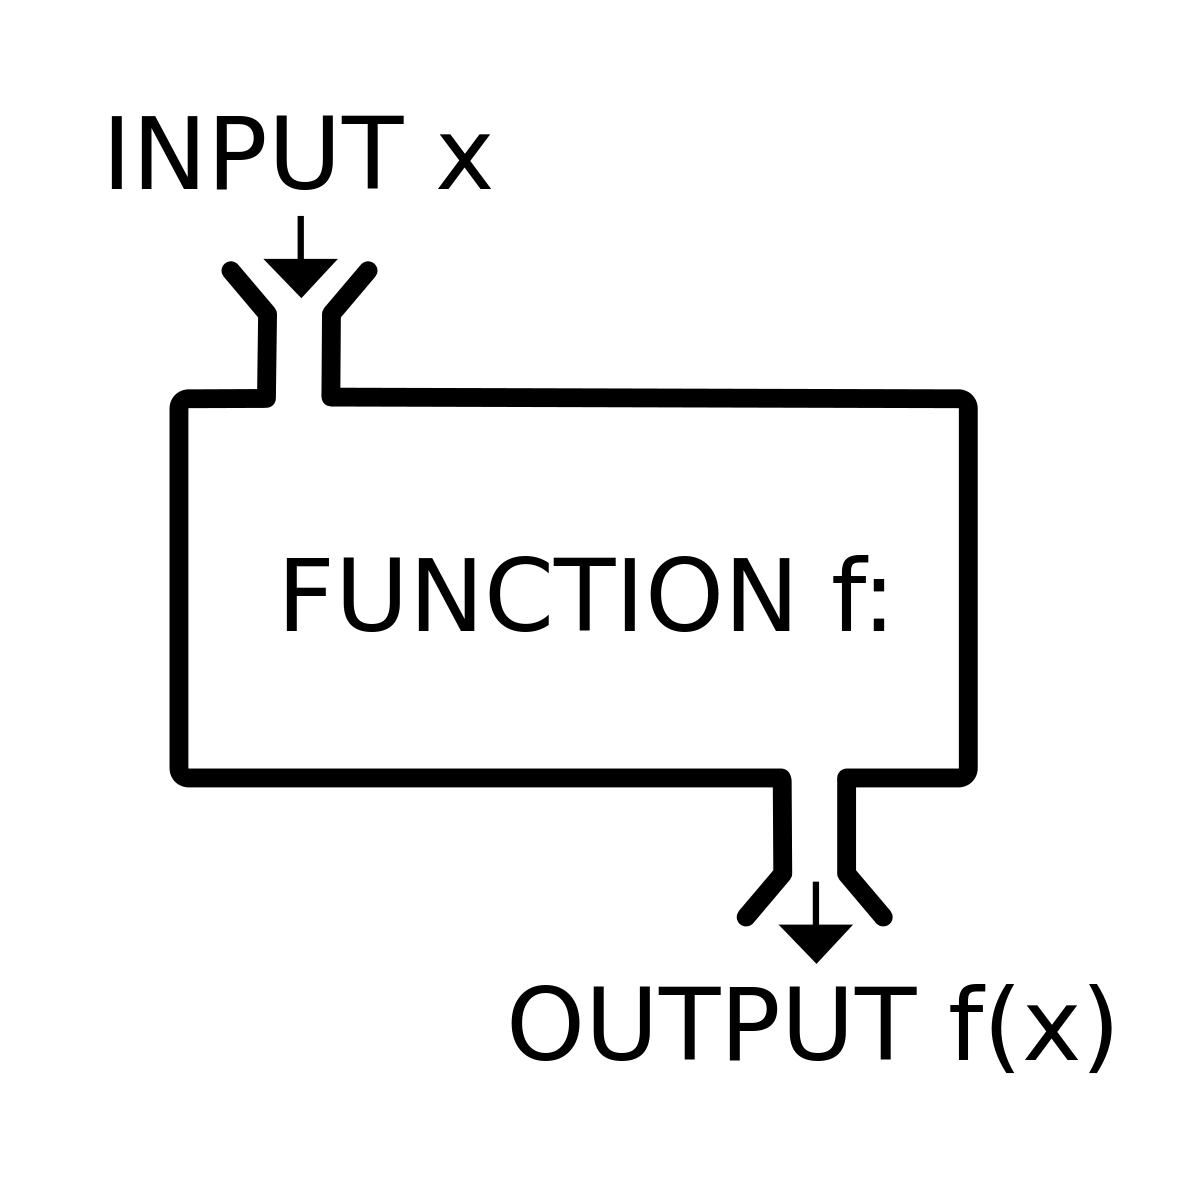
\includegraphics[width=0.7\linewidth]{images/bb.png}
    \end{center}
\end{figure}
\end{frame}


\subsection{Examples}

\begin{frame}[fragile]{You have already seen some functions.}{}
    \begin{itemize}
        \item main()
        \item sqrt(81)
        \item setup()
        \item draw()
        \item ellipse(50. 60, 10, 10)
        \item fill(255)
    \end{itemize}
\end{frame}

\begin{frame}[fragile]{The ellipse function.}{}
    \LARGE
    \begin{block}{Inputs to the ellipse() function}
        Coordinates of center. Size of ellipse.
    \end{block}
        \pause
    \begin{block}{What does the ellipse() function do ?}
        \pause
        Draws an ellipse on the screen, with specified parameters.
    \end{block}
        \pause
    \begin{block}{How ?}
        \pause
        Who cares ? . . .
    \end{block}
\end{frame}

\begin{frame}[fragile]{What do all functions have in common ?}{}
    \begin{itemize}
        \item main()
        \item sqrt(81)
        \item draw()
        \item ellipse(50, 60, 10, 10)
        \item fill(255)
    \end{itemize}
    \vfill
    \Huge Parentheses ()
\end{frame}


\subsection{Defining Functions}
\begin{frame}[fragile]{The structure of a Function}{}
\begin{figure}
    \begin{center}
        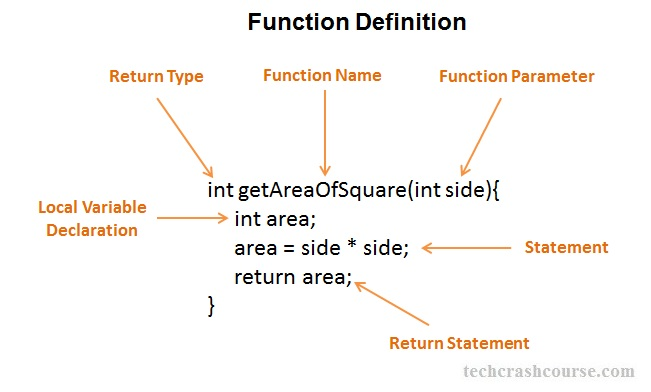
\includegraphics[width=0.8\linewidth]{images/func_label.jpg}
    \end{center}
\end{figure}
\end{frame}

\begin{frame}[fragile]{Control Flow}{}
\begin{figure}
    \begin{center}
        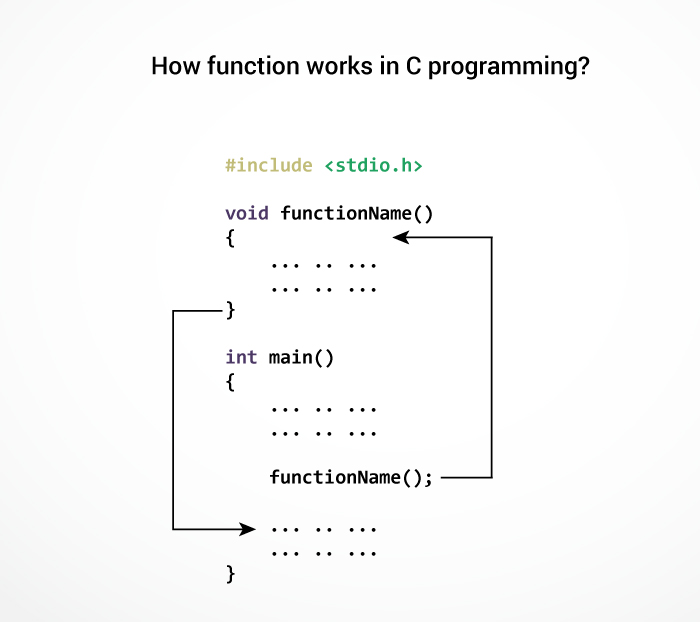
\includegraphics[width=0.8\linewidth]{images/func_flow.jpg}
    \end{center}
\end{figure}
\end{frame}

\begin{frame}[fragile]{Input to a Function}{}
\begin{figure}
    \begin{center}
        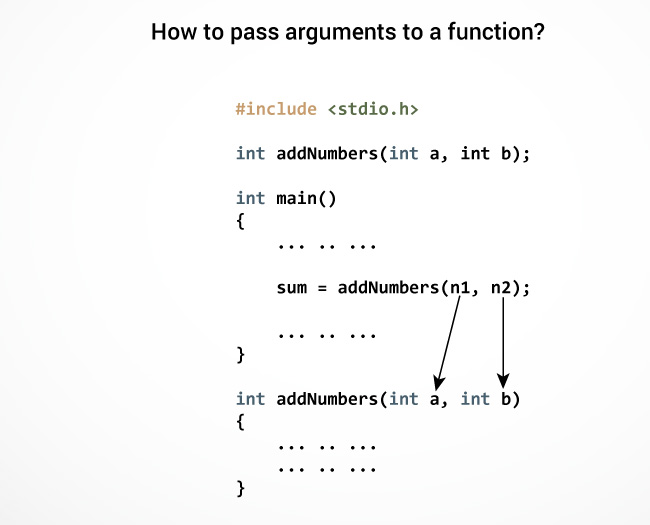
\includegraphics[width=0.8\linewidth]{images/func_args.jpg}
    \end{center}
\end{figure}
\end{frame}

\begin{frame}[fragile]{Return Value (output) of a Function}{}
\begin{figure}
    \begin{center}
        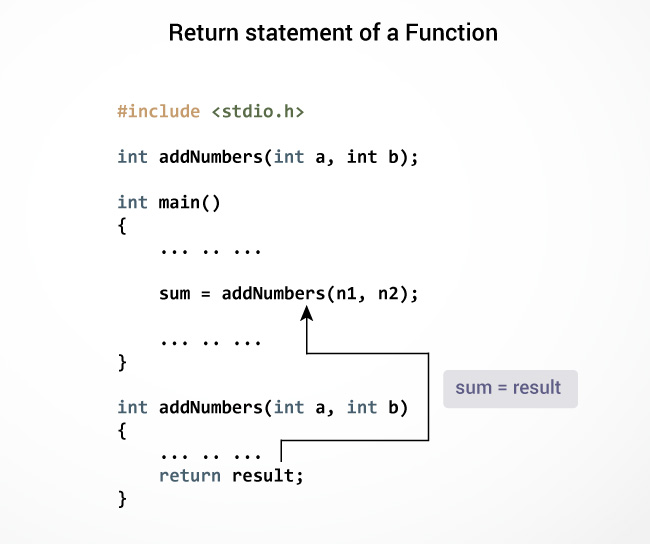
\includegraphics[width=0.8\linewidth]{images/func_return.jpg}
    \end{center}
\end{figure}
\end{frame}

\begin{frame}[fragile]{Exercise}{}
    \large
    \begin{block}{}
    Write a function drawTarget(), that takes $x$ and $y$ coordinate as input,
    and displays a target (concentric black and white circles) in that location.
    \end{block}
    \begin{block}{}
    Modify this function to take one integer N as input, and draw a target with N circles.
    This means that drawTarget(5) should display a target with 5 concentric circles.
    \end{block}
    \begin{block}{}
        Use this code to test.
        \begin{minted}{c++}
    void draw () {
        if (mousePressed) {
            drawTarget(mouseX, mouseY);
            delay(200);
        }
    }
        \end{minted}
    \end{block}
\end{frame}
